\documentclass[11pt]{article}
\usepackage{tikz}

\usetikzlibrary{arrows}

\begin{document}

\subsection*{Fsm for receiver}
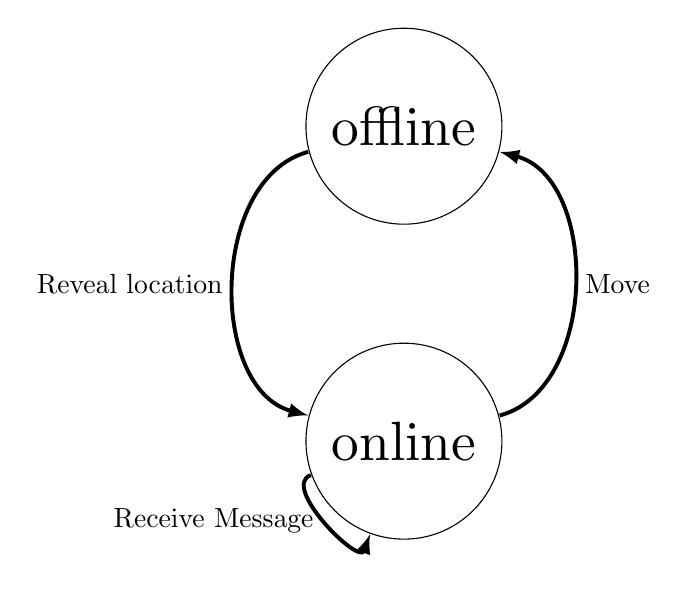
\begin{tikzpicture}
\node[draw, circle, scale=2] at (0,4) (off) {offline};
\node[draw, circle, scale=2] at (0,0) (on) {online};
\draw[arrows={-latex}, line width=.5mm, scale=2] (off) to [out=195, in=165]
  node[left] {Reveal location} (on);
\draw[arrows={-latex}, line width=.5mm, scale=2] (on) to [out=200, in=250]
  node[left] {Receive Message} (on);
\draw[arrows={-latex}, line width=.5mm, scale=2] (on) to [out=15, in=-15]
  node[right] {Move} (off);
\end{tikzpicture}

\subsubsection*{Reveal location}
\subsubsection*{Receive Message}
\subsubsection*{Move}

\end{document}
